\chapter{Background and Related Works}
\label{chap:Background}

In this chapter we review the relevant concepts to this study and introduce the techniques used during this research work.

\section{Stereo Vision}

Stereo vision is the concept of viewing a scene (object) in the real world from slightly different
viewpoints at the same time which results in stereo image pairs that are used by the human visual system or computer vision techniques to convey
depth in a scene. 

Using computer vision techniques, it is possible to extract depth information from stereo
images. This process is called {\it Stereo Matching} or {\it Stereo Correspondence} in computer vision,
which in fact leads to the construction of a
3D model of a scene from two or multiple views by finding corresponding pixels and therefore, their spatial displacement within various views of the same scene \cite{sze11}.

Corresponding pixels in stereo images are the ones that represent the same point in the real
world. As it will be seen shortly in more detail, the amount of horizontal motion of such pixels
in stereo pairs, which is referred to as {\it disparity}, is inversely proportional to the
distance from the observer, i.e., depth; however,  estimation of the exact depth of the points requires some
other information as well, such as the position, and the calibration data of the cameras that were used to take the pictures.
While the physical and geometrical approaches to this problem are well understood by researchers in the field, the process of finding the corresponding pixels correctly, 
yet efficiently, and measuring the disparity to generate a dense depth map still remains a challenging task. \newline

\section{Epipolar Geometry}
Understanding the fundamentals of the underlying geometry of stereo matching helps to better understand the principal idea behind all the methods designed to address this problem, 
thus facilitating the comprehension of 3D model reconstruction from stereo image pairs. Therefore, we will thoroughly describe the basic geometry of stereo matching in this section. \newline
If we consider two cameras that are looking at a particular scene from slightly different view points, 
a back projection of any point in the 3D space via rays passing through each camera centre,
${C}^{'}$ and ${C}^{"}$, would result in two distinct points on each image plane. For simplicity, we will refer to the point 
in space as $P$, and its projection on the first (left) and second (right) image planes,
as $P^{'}$ and ${P}^{"}$ respectively. \newline
As a result of $P$'s back projection on the image planes, an important property will emerge between the points and the camera centres, which is coplanarity of all these points. 
This plane, also referred to as {\it epipolar plane}, passes through $P^{'}$, $P^{"}$ and the camera centres, thus intersecting each image plane. 
It should be noted that this property, from which the consequent properties are derived, is the building block of stereo matching methods. 
Let us denote the specified plane by $S$ for further reference. 
Since $S$ passes through the camera centres, it clearly traverses the line 
that connects two camera centres. This line, which is known as the {\it baseline}, intersects each image plane at a point called the {\it epipole}; denoted by ${e}^{'}$ and ${e}^{"}$
in Figure \ref{fig:epg}. 
Consequently, the intersection of the plane $S$ and each of the image planes, creates a line called {\it epipolar line} \cite{hart2000}. 
The {\it epipolar line} always passes through the {\it epipole} in the image plane. 
These concepts, illustrated in Figure \ref{fig:epg}, constitute the important components of the stereo correspondence geometry.

\begin{figure}[!h]
\centering
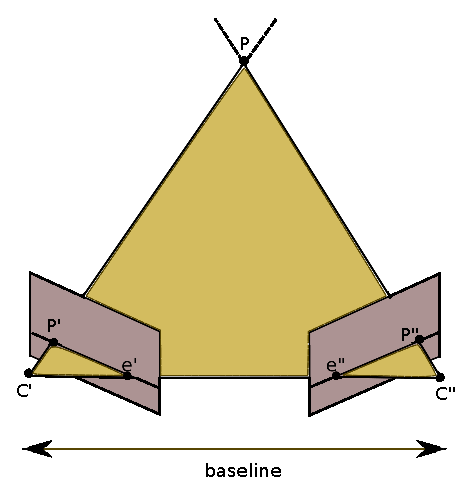
\includegraphics[width=0.5\textwidth]{epipole}
%\includesvg{epipole}
\caption{Epipolar geometry}
\label{fig:epg}
\end{figure} 

Now, we can define the problem of stereo correspondence as a case in which the location of $P^{'}$ in the image plane is known, while the
corresponding point $P^{"}$ is unknown; therefore, the problem can be stated as an attempt to find the correspondence of $P^{'}$ in the second image plane. Based on the aforementioned 
properties, we know that $P^{"}$ is located somewhere on the line, the epipolar line,
created by the intersection of the plane traversing the ray that goes through $P^{'}$ and the first camera centre and the {\it baseline}. This line is in fact, the projection of the ray going
through $P^{'}$ and the first camera centre, on the right image plane. Therefore, the search for the corresponding point, $P^{"}$, will be limited to merely scanning the corresponding 
epipolar line on the second image plane rather than the whole image.

%\begin{figure}{h!}
%\centering
%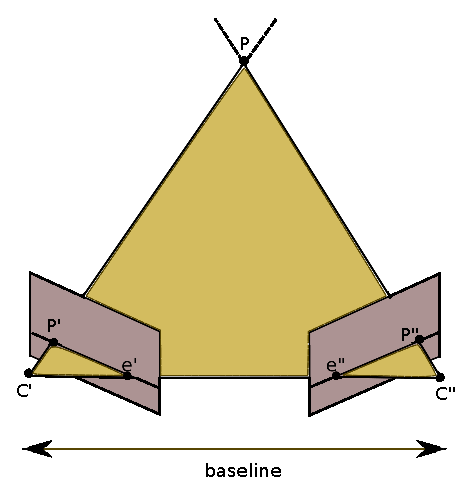
\includegraphics[width=1.5in,height=1.5in]{epipole}
%\end{figure}

It is now apparent that in order to find the correspondence of a particular point $P^{'}$, in the second image plane
the corresponding epipolar line, must first be sought. 
The projection from a point to its corresponding epipolar line can be obtained through certain transformations in space; normally a rotation and translation, Figure \ref{fig:rectify}.
For further geometrical calculations, these transformations can be represented
with a matrix that is only dependant on the camera's properties, not the scene \cite{hart2000}.
However, dealing with these transformations while looking for the corresponding points, can increase the complexity of stereo matching algorithms to certain levels \cite{sze11}; therefore, 
in order to avoid this issue, many stereo matching approaches are proposed based on the assumption that image pairs are first warped \cite{sze11}.
This process is known as {\it image rectification} which is basically achieved by first having the cameras rotated in a way that their optical axis, 
the line passing through the camera centre which is perpendicular to the image plane, are parallel to each other; 
that is their optical axis is perpendicular to the baseline. As a result of this transformation, the epipoles are sent to infinity. 
Furthermore, it might be necessary to have the cameras tilted so that their {\it y} axis also becomes perpendicular to the optical axis. 
After these two steps, corresponding epipolar lines actually become horizontal scanlines; Figure \ref{fig:rectify}. This pre-processing step significantly constrains the process of searching 
for corresponding points and eliminates certain complications in stereo matching algorithms \cite{sze11}.

\begin{figure}[!h]
\centering
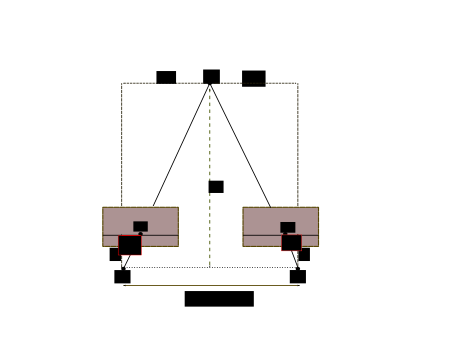
\includegraphics[width=0.65\textwidth,trim=22mm 0mm 0mm 150mm,clip]{rectdisp}
\caption{Rectified image pairs and disparity geometry}
\label{fig:rectify}
\end{figure} 

Sample stereo images taken using two regular webcams are displayed in figures \ref{fig:unrect} and \ref{fig:rect},
before and after rectification. 
The red line shows how features get aligned in the left and right image after the rectification process.

\begin{figure}[h!]
\centering
\subcaptionbox{Left image unrectified}
[.5\linewidth]{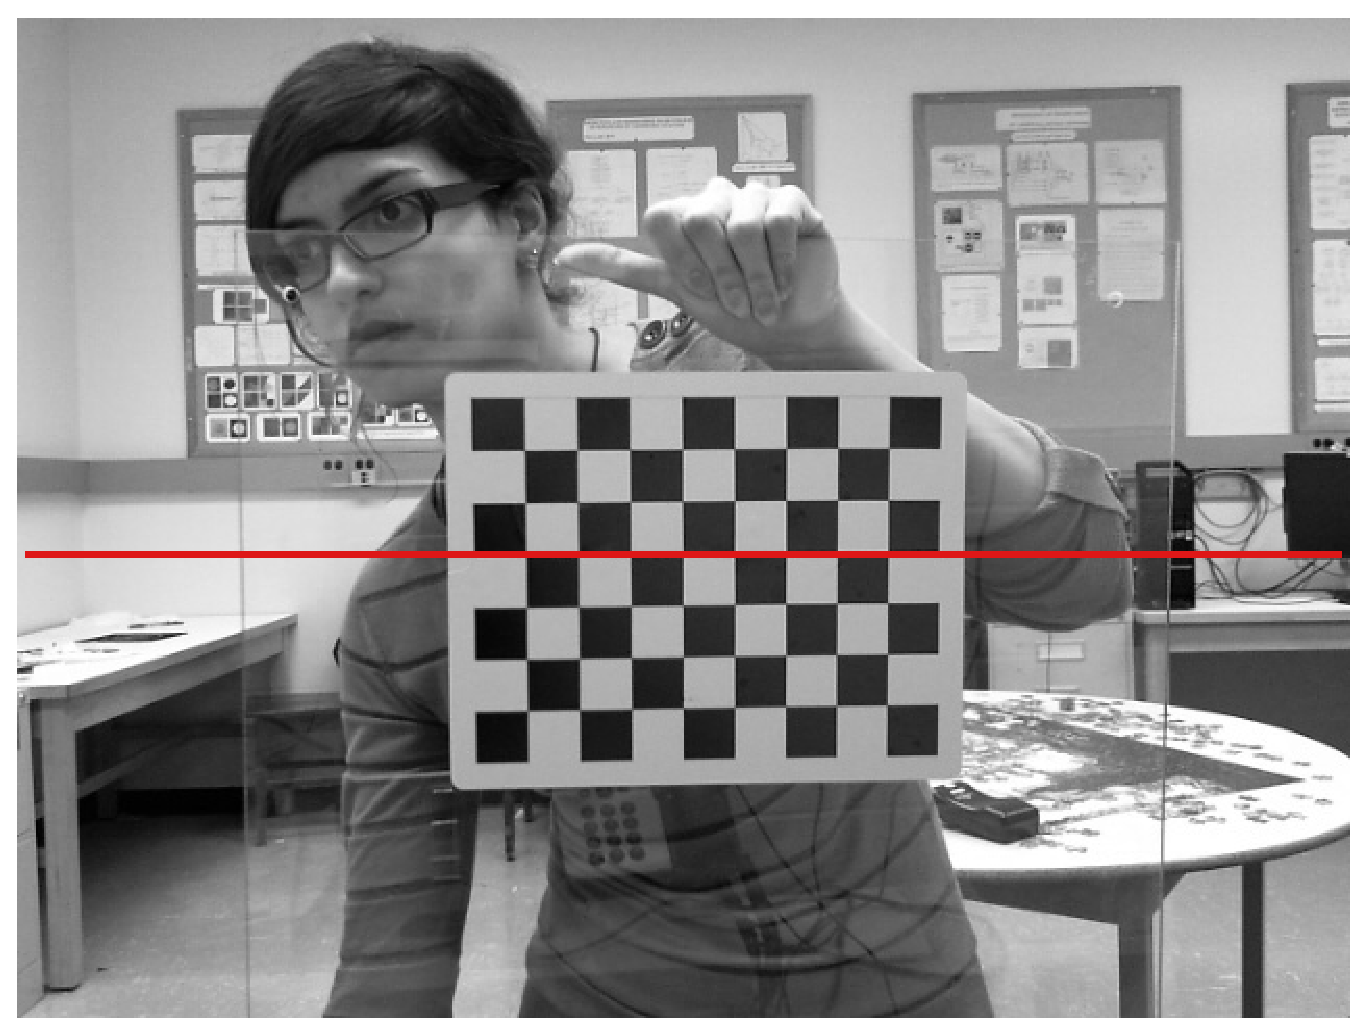
\includegraphics[scale=0.35]{RectL}}%
\subcaptionbox{Right image unrectified}
[.5\linewidth]{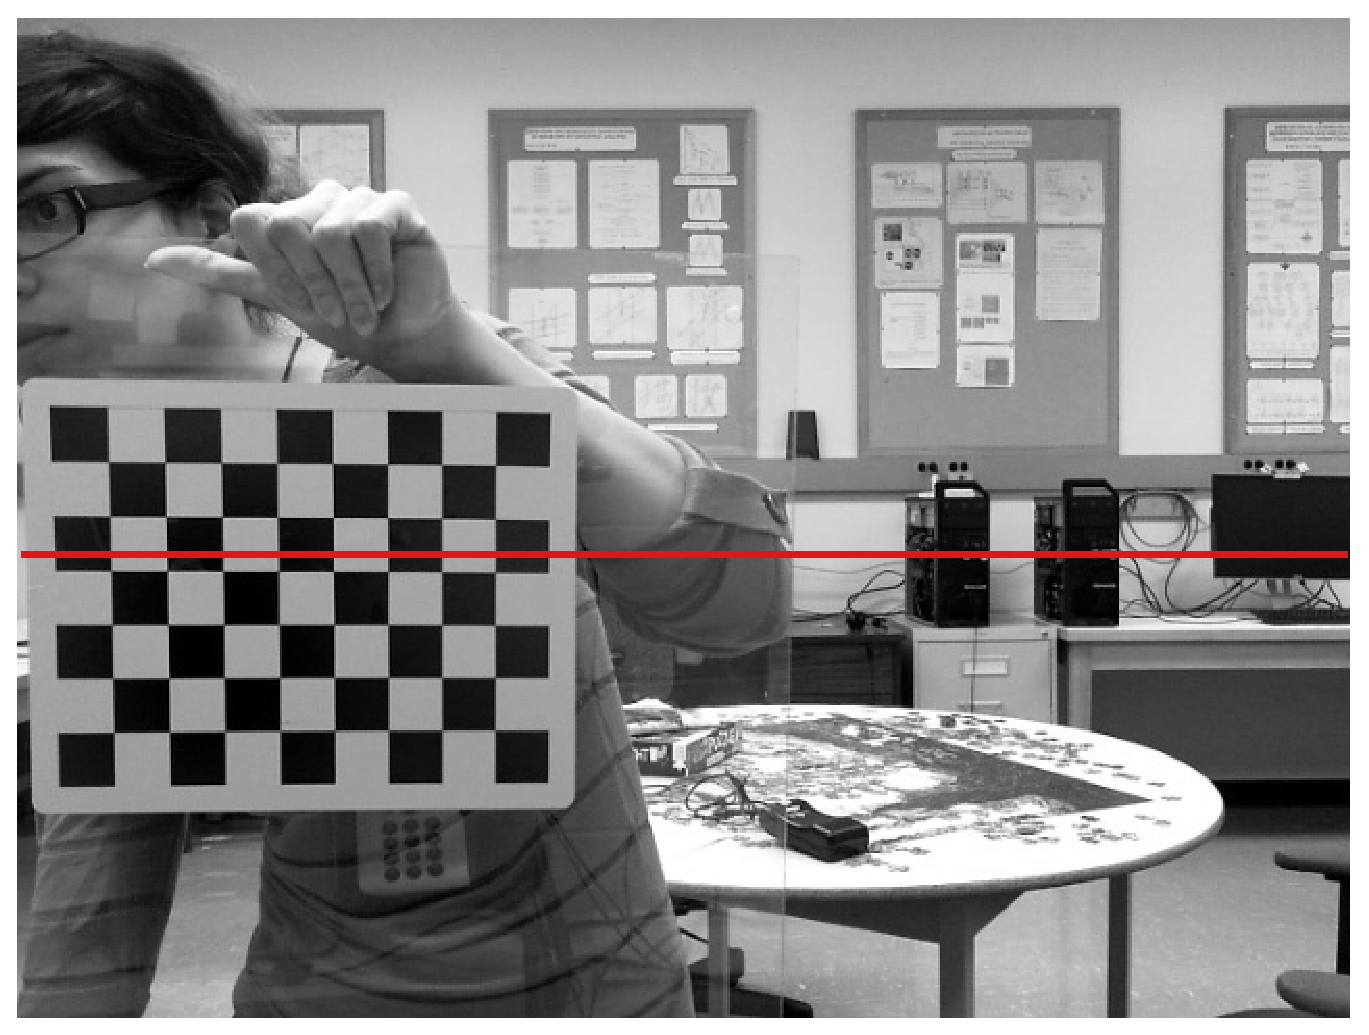
\includegraphics[scale=0.35]{RectR}}%
\caption{Sample stereo image before rectification}
\label{fig:unrect}
\end{figure}

\begin{figure}[h!]
\centering
\subcaptionbox{Left image rectified}
[.5\linewidth]{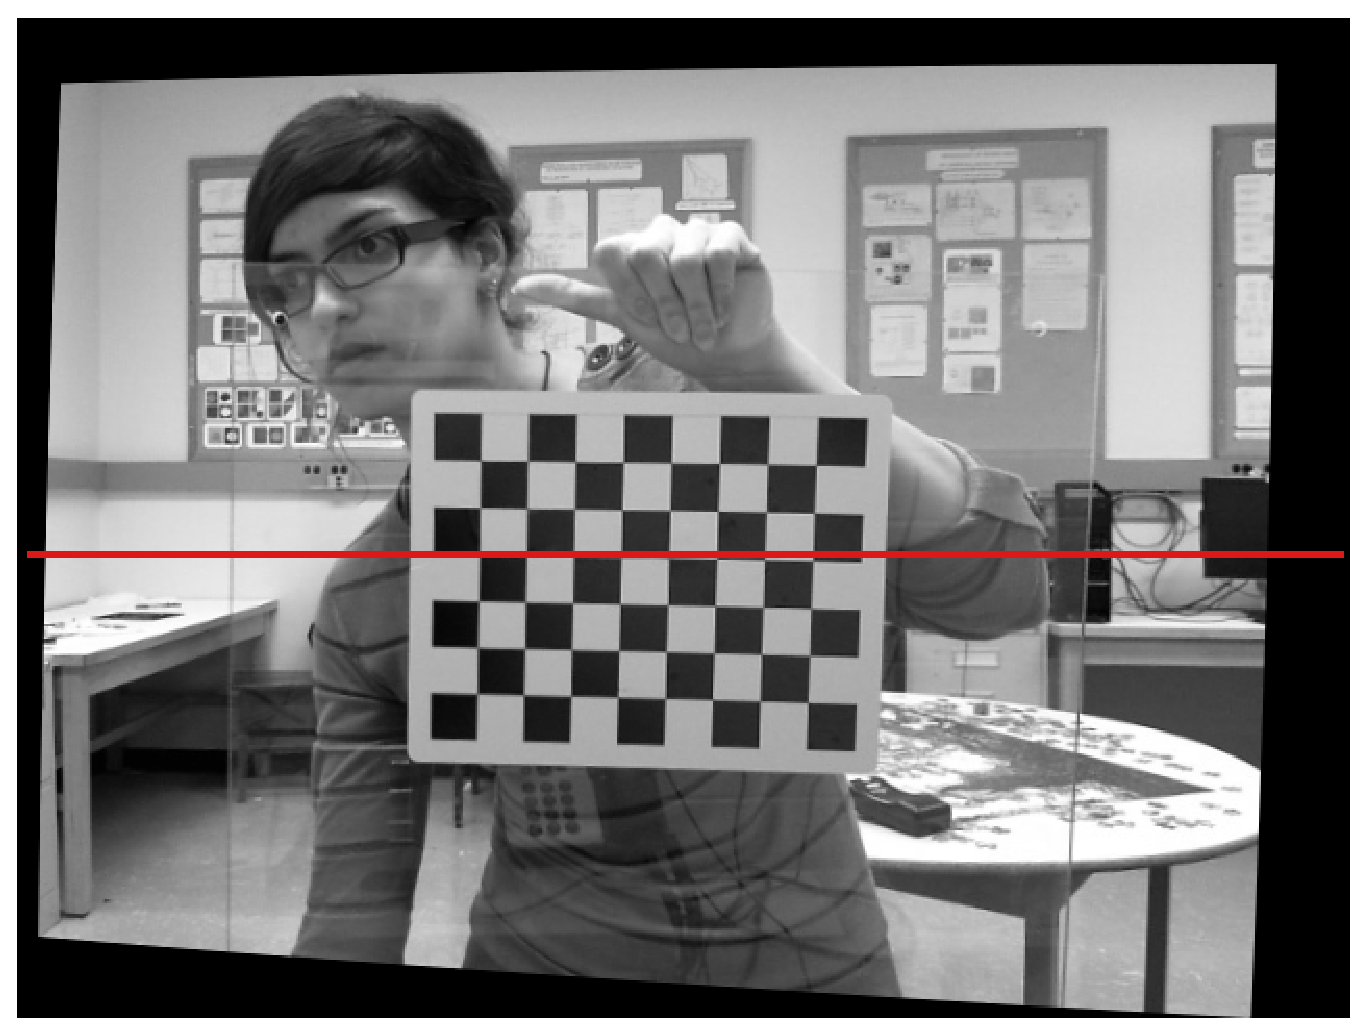
\includegraphics[scale=0.35]{rectLmark}}%
\subcaptionbox{Right image rectified}
[.5\linewidth]{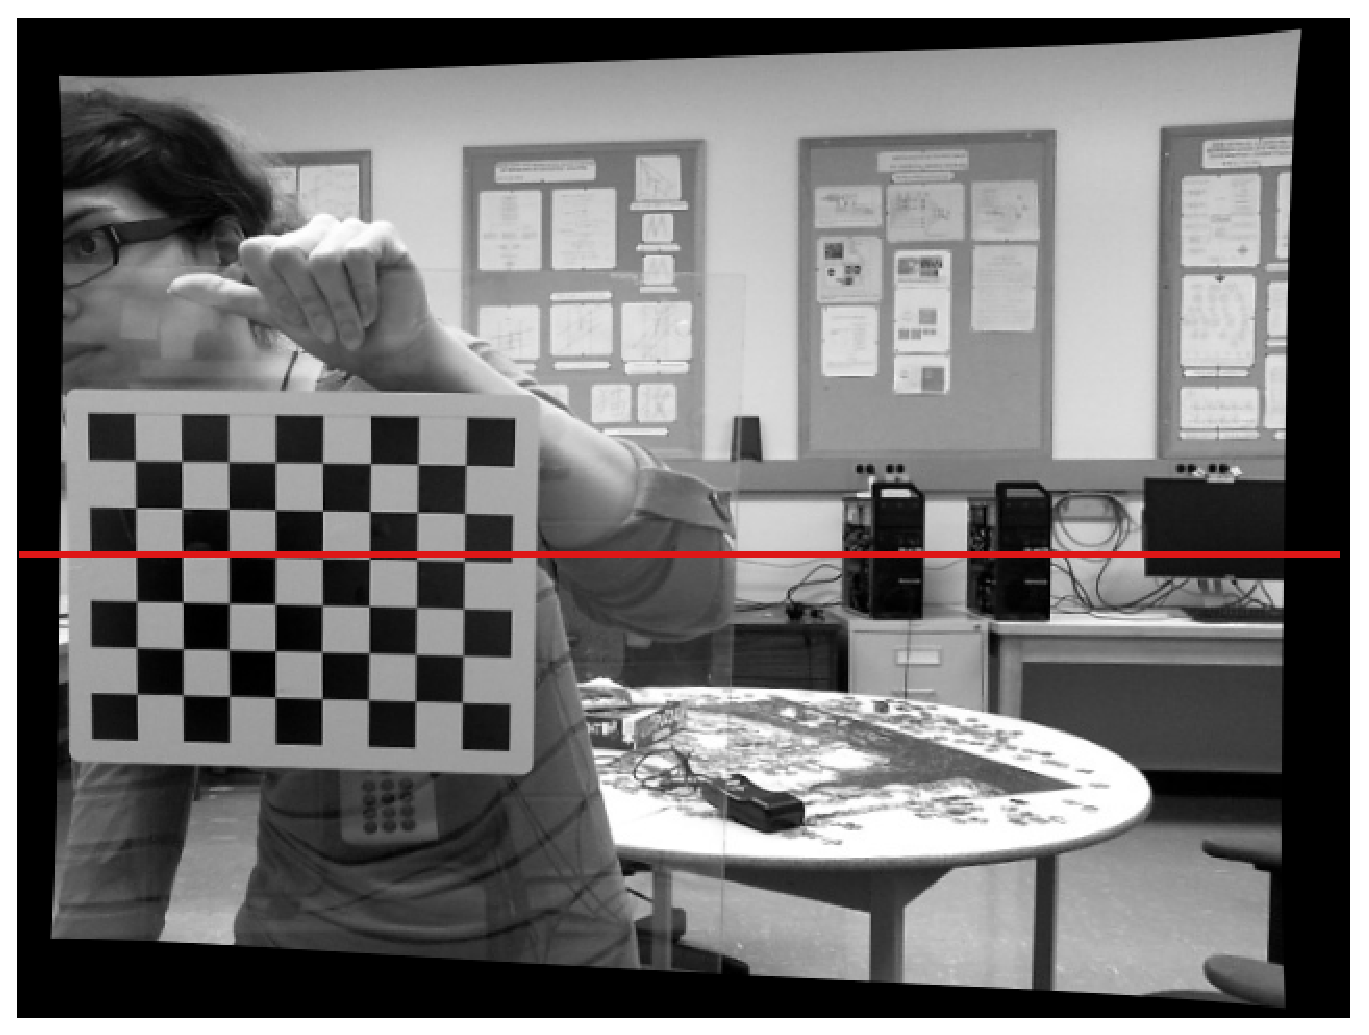
\includegraphics[scale=0.35]{rectRmark}}%
\caption{Sample stereo image after rectification}
\label{fig:rect}
\end{figure}

Using the rectification model and epipolar geometry described earlier, 
derivation of the geometrical relation through which the depth of a certain point in 3D space 
can be obtained, will be straightforward. This relation is presented as follows \cite{sze11}:
\begin{align}
\frac{X_{L}}{Z} &= \frac{x_{l}}{f} \label{eq:1} \\
\frac{-X_{R}}{Z} &= -\frac{x_{r}}{f}  \Rightarrow B-\frac{X_{L}}{Z}=-\frac{x_{r}}{f} \label{eq:2} \\
(\ref{eq:1}) + (\ref{eq:2}) \Longrightarrow  \frac{B}{Z} &= \frac{x_{l}-x_{r}}{f} \label{eq:3} \\
\intertext{if $x_{l}-x_{r}=d$, we will have:}
d &= \frac{Bf}{Z} \label{eq:dispeq}
\end{align}
where f is the {\it focal length} measured in pixels, B is the {\it baseline}, Z is the {\it 3D depth}, and d is the {\it disparity}. The relationship between corresponding pixels in the left
and right images according to disparity {\it d} is also as follows:
\begin{align}
{P}^{"}_{x} &= {P}^{'}_{x}+d(x,y) \\
{P}^{"}_{y} &= {P}^{'}_{y}
\end{align}
Therefore, based on the aforementioned formulas, the depth of points in 3D space can be easily calculated after finding the corresponding pixels in multiple views and consequently their
disparities \cite{bol87,oku93,sch02}.

\section{Stereo Correspondence Algorithms}
A survey of the field shows that the algorithms which address stereo correspondence problem can be roughly divided into two main classes \cite{sch02}. These classifications are commonly known as:
\begin{enumerate}
\item Sparse Correspondence Algorithms
\item Dense Correspondence Algorithms 
\end{enumerate}

Regardless of the category, stereo matching algorithms normally include specific steps in the process of finding the corresponding pixels in the stereo images.
According to the taxonomy by Scharstein et al. these steps are as followed:

\begin{enumerate}
\item {Calculation of matching cost}
\item {Aggregating the costs}
\item {Disparity computation}
\item {Disparity refinement}
\end{enumerate}

Depending on each algorithm, these steps and their sequence may change.

In this section, we are going to briefly describe the important specifications of the algorithms belonging to each of these two categories.
\subsection{Sparse Correspondence Algorithms}
Sparse correspondence algorithms, also known as feature-based algorithms, are the early stereo matching methods. In the 1980s, this class of algorithms received considerable attention by
many researchers in computer vision \cite{dhon89}.
In this type of methods, particular features in an image, such as edges, 
points, line segments, or other distinctive features are extracted; therefore, the search for corresponding pixels is only applied to these regions. 
Consequently, algorithms of this
sort result in a sparse disparity map \cite{matt89,hsie92, sze11}. The introduction of feature-based algorithms has mainly been motivated by three important factors \cite{bro03,sze11}:
\begin{itemize}
\item Lack of advanced hardware and technology for exhaustive computational tasks.
\item Constraint of the search area in order to find more reliable matches.
\item Stability of particular features to look for correspondences under certain circumstances where the image pairs are affected by external factors, 
such as illumination variations; in other words, when there is a considerable difference in photometric properties between the images pairs, 
particular features such as the edges may be more reliable to start the correspondence search.
\end{itemize}

However, the requirement of having dense depth maps for many applications and also the emergence of efficient {\it dense correspondence algorithms}, have diverted the attention away
from this class of algorithms in the last 20 years.

\subsection{Dense Correspondence Algorithms}
Unlike feature-based methods, dense correspondence algorithms try to find the
correspondences for all the pixels in the image, and therefore, result in a dense disparity map. Most recent algorithms and studies have focused on this class of algorithms since many applications 
nowadays, such as graphical rendering, 3D model construction, or augmented reality require a dense depth map of the scene. 
However, these algorithms face many challenges that need to be properly
addressed, such as finding the depth values in occluded regions, depth discontinuities, and textureless areas \cite{sch02,bro03}.

Dense correspondence algorithms are usually classified in two groups based on how they assign
disparities to pixels \cite{sze11}:
\begin{enumerate}
\item Local approaches
\item Global approaches
\end{enumerate}

\subsubsection{Local Approaches} 

Local methods tend to find the disparity of each pixel based on its neighboring pixels. In
other words, the disparity of a pixel is calculated in a finite window containing its neighboring pixels, based on a particular metric, e.g. the intensity values \cite{sch02}.

These methods make an implicit smoothness assumption for the pixels in the search
window, and therefore, assign the same disparity to all the pixels belonging to the same window which could result in incorrect disparity values in slanted surfaces or
depth discontinuities \cite{hirsch02}. This assumption can be considered as one of the major drawbacks of local methods.
Another drawback of local methods is their dependency on the window size \cite{sch02}. A fixed window size can raise certain problems in these algorithms:
\begin{enumerate}
\item If too large of a window size is considered, due to aforementioned smoothness assumption, the algorithm may result in blurry object boundaries and inaccuracy near depth discontinuities.
\item If the selected window size is too small, the disparity values will be less accurate and harder to find since little information has been considered for 
finding the correspondences of pixels in the image.
\end{enumerate}

However, a significant advantage of using local approaches is their high speed in finding disparity results.\newline

\subsubsection{Global Approaches}
Unlike local approaches, in global methods the disparity of a pixel depends on the information in
the whole image. Global methods usually include an optimization step of a global energy
function\cite{roy98,bobi99,boyk01,hong10}. In this class of algorithms, an optimal disparity value for each pixel is sought that leads to minimization of a global cost
function that normally combines a data term with an explicit smoothness assumption.

\begin{equation}
E(d)=E_{data}(d)+\lambda E_{smooth}(d)
\end{equation}
The term $E_{data}$ is normally defined as the difference of a common metric, e.g. the photometric property, between the corresponding pixels and is denoted as follows:

\begin{equation}
E_{data}(d) = \sum_{(x,y)}C(x,y,d(x,y))
\end{equation}

where C is a matching cost. The matching cost function can have various definitions depending on the algorithm; however, as mentioned above, it is normally defined as sum of absolute difference 
between the intensity of the corresponding pixels in two images \cite{sch02}.

The term, $E_{smooth}$, is the smoothness assumption based on which the disparity values in different regions are refined. The definition of this term can also vary in 
different solutions. $\lambda$ is also a weighting factor, by which the effect of the smoothness assumption in the global function can be controlled in the algorithm \cite{sze11}.
In order to find the minimum of the global function, certain approaches in computer science have proved to be particularly useful. 
To name some of these approaches, we can refer to dynamic programming \cite{kim05}, graph cut \cite{boy01,boyk01,boy04}, and belief propagation \cite{sun11}. 
Many researchers have studied and addressed the problem of stereo matching
by applying one of these approaches.

The major drawback of global approaches is normally their high usage of computational resources and low speed. However, 
they usually result in more accurate disparity values \cite{hirsch02,sze11}. 

It is also worthwhile to mention that in the past twelve years, another group of algorithms have emerged which cannot be explicitly classified in any of the previously mentioned groups.
These methods, which are known as {\it Segmentation-based techniques}, first segment the image into regions and then, rather than searching for correspondences per pixel,
they attempt to find the corresponding disparity for each region. A more detailed review of these methods can be found in chapter 11 of \cite{sze11}.

\section{Edge Detection}

As mentioned earlier in the ``Introduction'', salient {\it edges} in the scene are one of the important features 
that can be used in many applications, such as object detection, image stitching, or 3D model reconstruction.
Due to their importance and application in this research, we review some of the relevant concepts and techniques in computer vision in this section.

\subsection{Edges}
When looking at a scene, an edge is defined whenever the visual system can perceive a distinguishable variation in color, intensity or texture between 
different regions \cite{sze11}.
Therefore, a reasonable mathematical approach to detect the edges in an image would be calculating the gradient of the intensity image and then looking for the maximum
values. Another alternative would be getting the second derivative of the image and then looking for zero values. However, since an image is normally affected by a 
certain amount of noise which intensifies at higher frequencies, taking the derivatives of the image can lead to significant noise amplification, 
as it makes high frequency signals more prominent to others.
Therefore, it is better to attenuate high frequencies prior to applying any edge detection approach. 
There are a variety of filters for image smoothing (blurring); however, since we want to attenuate high frequencies, it is better to use a low-pass filter, which only passes low frequencies.
A widely known class of image blurring filters in computer vision are called {\it linear filters}, whose output is a linear function of their input. 
In linear filtering operators, for each pixel a weighted summation of its neighboring pixels
is used in order to estimate its final value \cite{sze11}. In mathematics, this process can be modelled by convolution of the input signal with a particular function, known as kernel. 
\begin{equation}
g(i,j)=\sum_{k,l}f(i+k,j+l)h(k,l)
\end{equation}
which is denoted as:
\begin{equation}
g=f\bigotimes h
\end{equation}
where $f$ and $g$ are the input and output signals respectively, and $h$ is the kernel function which can vary depending on the type of filter. 

Therefore, each filter can modify the input signal differently based on its corresponding kernel function.
The Gaussian filter is a filter commonly used for attenuating higher frequencies in an image and filtering out the noise \cite{wells86}. 
Since edges in an image may be oriented along any arbitrary direction, 
applying a filter which is biased towards a particular direction in filtering out the noise, would not be a prudent decision. Instead, a better choice would be choosing a filter 
with a symmetric 2D kernel function. 
This feature is particularly found in the Gaussian filter, since it employs a 2D symmetric kernel. Because of this unique feature, 
the Gaussian filter is normally used in most edge detection algorithms as a pre-processing step.
An isotropic, i.e. circularly symmetric, the Gaussian kernel has the following form \cite{sze11}:
\begin{equation}
G(x,y)=\frac{1}{2\pi \sigma ^{2}} e^{-\frac{x^{2}+y^{2}}{2\sigma^{2}}}
\end{equation}
where $\sigma$ is the standard deviation. 
A more thorough description of the Gaussian and some other types of filters can be found in chapter 3 of \cite{sze11}.

After smoothing the image with the Gaussian filter, the gradient of the smoothed image should be taken in order to detect the edges. This can be done by convolving 
the signal with a pair of convolution masks in each direction in order to detect the edges, both horizontally and vertically. An edge extracting operator called {\it Sobel} is normally used
for this purpose \cite{sze11}. 
Sobel convolution kernels for both x and y directions are defined as follows \cite{sze11}:

\begin{align}
G_{x} &= \begin{bmatrix}
-1 & 0 & +1 \\ 
-2 & 0 & +2 \\ 
-1 & 0 & +1
\end{bmatrix} \\
G_{y} &= \begin{bmatrix}
-1 & -2 & -1 \\ 
0 & 0 & 0 \\ 
+1 & +2 & +1
\end{bmatrix}
\end{align}

Following the estimation of image gradients in each direction, the magnitude and the direction of an edge element can then be found by \cite{sze11}:
\begin{align}
\left | G \right | &= \sqrt{G_{x}^{2} + G_{y}^{2}} \\
\theta &= \arctan (\frac{G_{y}}{G_{x}})
\end{align}

The process of applying the Sobel operator mask \cite{sobel78} to the smoothed image, is in fact equivalent to getting 
the first or second order directional derivative of the smoothed image \cite{sze11}. As a result of this process, edge elements are detected throughout the image.
After finding the edge points, the next step would moving along the edge direction and suppressing, setting to zero, any point which is not an edge.

The {\it Canny} edge detector, proposed by John F. Canny in 1986 \cite{canny86}, is one of the most commonly used edge detection approaches. In addition 
to the process described above for detecting the edges in the image, two different thresholds are defined in the process. 
The purpose of having these two thresholds is the elimination of streaks, which are the breakage along an edge contour, which is caused by the signal fluctuating around the threshold.
Using these thresholds in the process of edge detection, any value above the higher threshold will be output as an edge element and while inspecting other pixels along 
the edge direction, only those values above the lower threshold will be accepted \cite{canny86}.
This process has shown to reduce the streaking effect to a significant amount \cite{canny86}. \newline
Figure \ref{fig:edgenodil} shows the detected edges obtained by applying the canny operation on the image \ref{fig:imggt5}.

\begin{figure}[H]
\centering

\includegraphics[scale=0.35]{imggt5}
\caption{Canny edge detection in an image}
\label{fig:imggt5}
\end{figure} 

\begin{figure}[H]
\centering
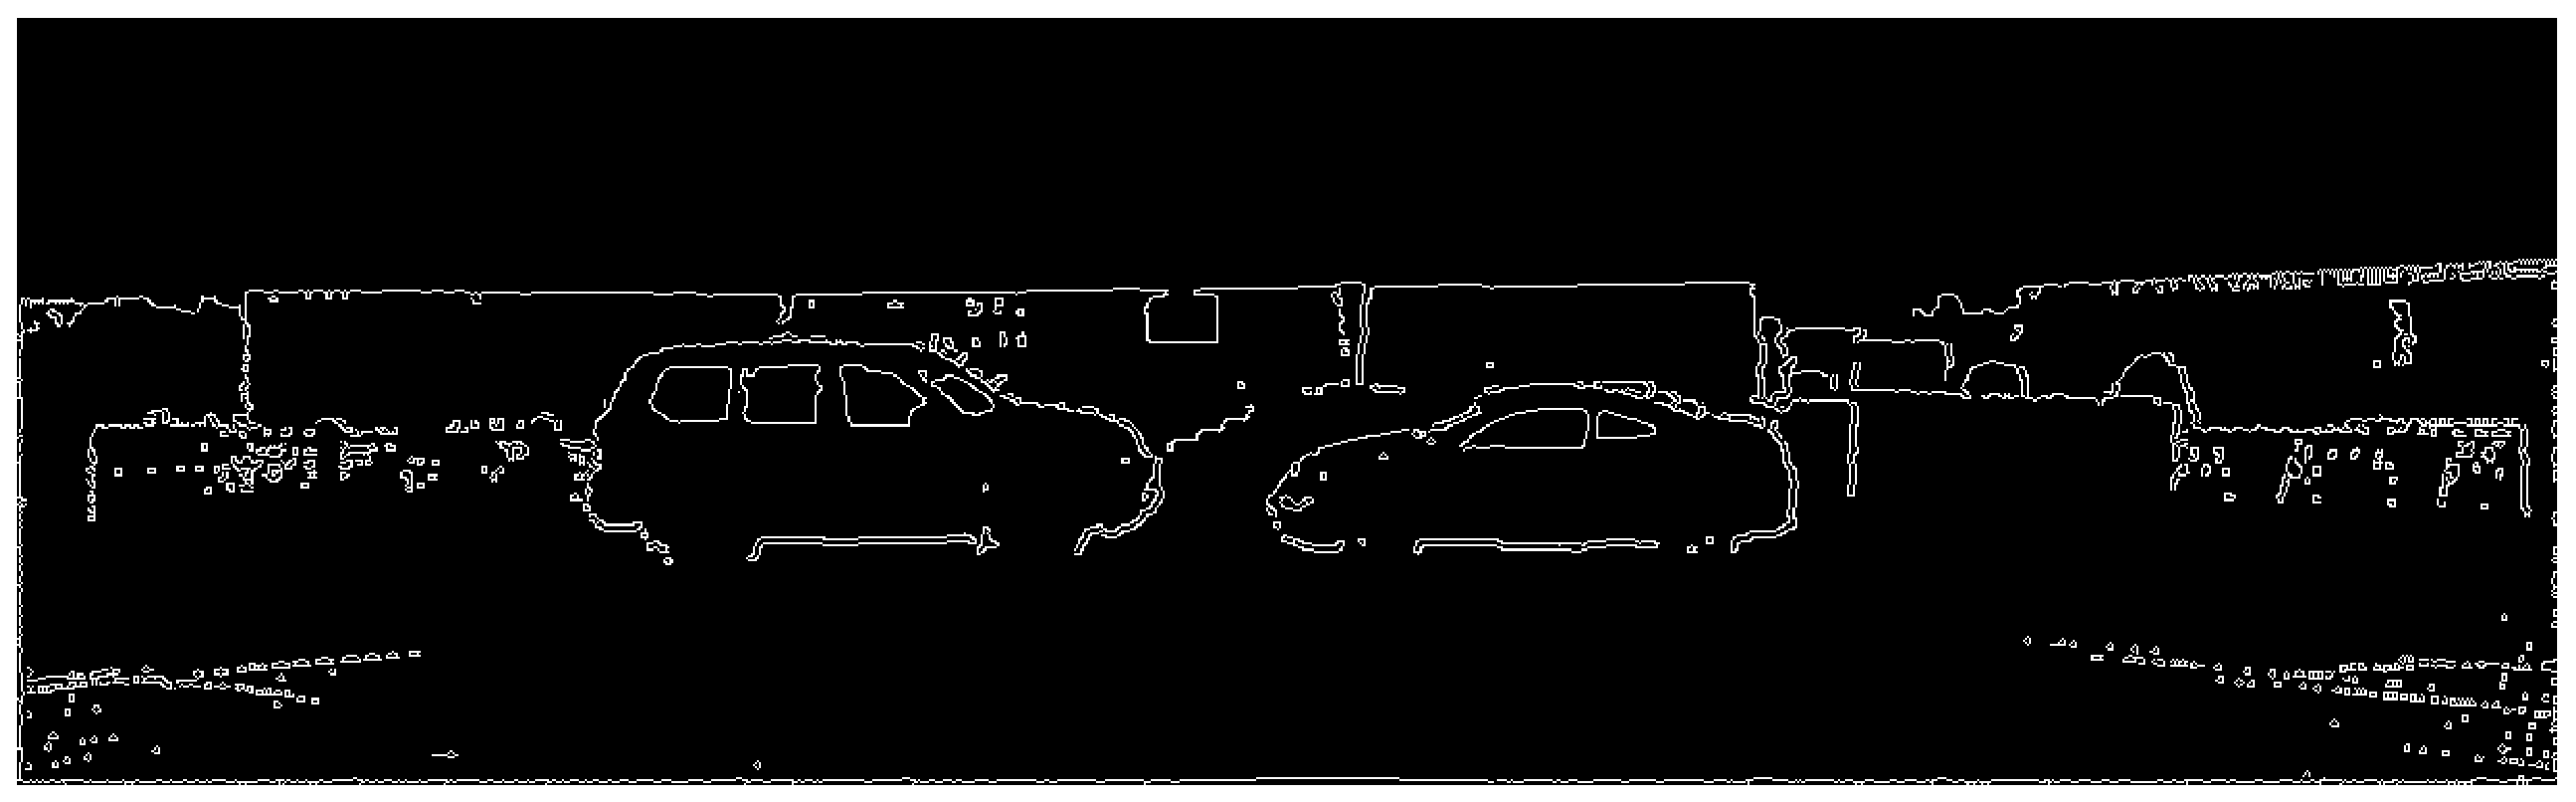
\includegraphics[scale=0.35]{mask5nodil}
\caption{Canny edge detection in an image}
\label{fig:edgenodil}
\end{figure} 

\section{Morphological Operations}
In addition to linear filters, there is another type of filters known as {\it non-linear filters}, whose output is a non-linear function of their input. 
In this type of filtering, unlike linear filters, the final value of a pixel is not necessarily 
a weighted combination of its neighboring pixels \cite{sze11}. 
{\it Median filter, Bilateral filter}, and {\it anisotropic diffusion} are all different types of non-linear filters. Non-linear filters are used for certain image manipulation 
and enhancement tasks, and are commonly used with a particular type of image called {\it binary
image} \cite{sze11}. Binary images, as their name indicates, consist of merely two pixel values, 0 or 1. These images are usually the outcome of filtering the values in an image 
by a certain threshold, thus changing each value to 0 or 1 based on the comparison against the threshold. Binary images are
widely used for {\it masking} operations in image processing \cite{sze11}. Due to extensive application of binary images, certain operations are usually employed to manipulate them. 
These operations are known as {\it morphological operations} \cite{ritt00}.
In morphological operations, the original image is convolved with a {\it structuring element}, also known as kernel. 
The structuring element is a mask (a binary image), normally smaller than the original image, 
with which different structures can be defined for later modification of the image. 
{\it Dilation} and {\it Erosion} are two of the most basic and widely used morphological operations in binary image processing.
These two operation are normally used for expansion and erosion of the shapes in the original image. 
In dilation, the structure element which is usually in form of a circle or square with the origin located at its centre, is superimposed on top of the original binary image.
By moving the structure element over the background pixels, each pixel belonging to the background, that 
is overlain by the centre of the structuring element, is replaced by foreground value if at least one of the pixels of the structuring element coincide with any pixel marked as foreground.
Erosion, which can be considered as the complementary operation of dilation, follows a similar process, with only the difference that structuring element is moved over foreground pixels and any
foreground pixels will be replaced by the background value if at least one pixel of the structuring element overlaps with a pixel marked as background.
Hence, we can state that dilation of the foreground is equivalent to erosion of the background \cite{ritt00}.
The dilation and erosion operations are illustrated in figures \ref{fig:dilate} and \ref{fig:erode}, respectively.

\begin{figure}[H]
\centering
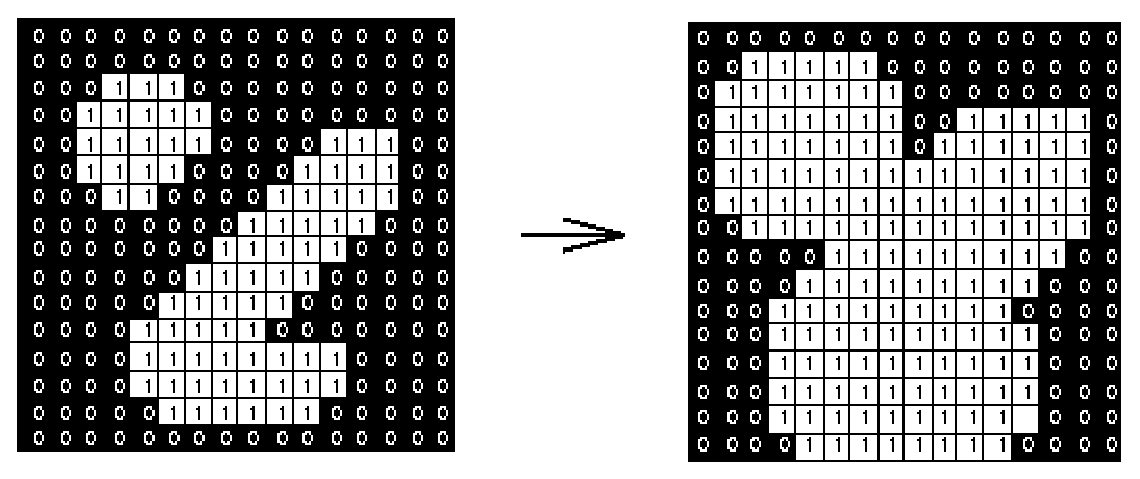
\includegraphics[scale=0.8]{diltbin}
\caption{Dilation operation \cite{HIPRdil}}
\label{fig:dilate}
\end{figure} 

\begin{figure}[H]
\centering
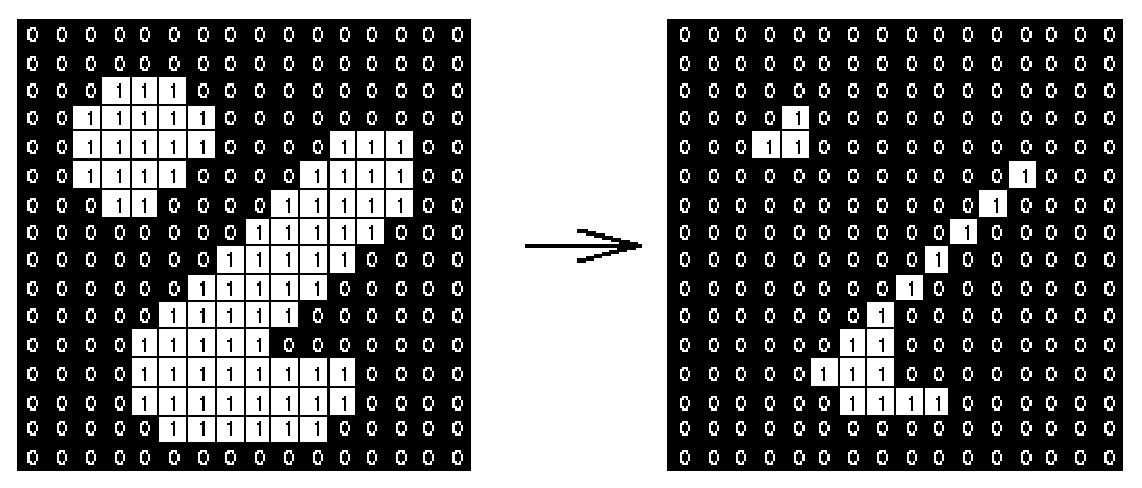
\includegraphics[scale=0.8]{erodbin}
\caption{Erosion operation \cite{HIPRerod}}
\label{fig:erode}
\end{figure} 

The sample image shown in figure \ref{fig:edgenodil} is presented below after applying dilation on the detected edges in the image to expand the 
detected regions.

\begin{figure}[H]
\centering

\includegraphics[scale=0.35]{mask5dil}
\caption{Dilation of the detected edges in an image}
\label{fig:edgedil}
\end{figure} 


